\myChapter{Implementacja}\label{ch:implementation}
%************************************************

\section{Oprogramowanie mikrokontrolera}
W pracy wykorzystany został układ \textsmaller{AVR Atmega8}, będący ośmiobitowym mikrokontrolerem. Sprzęt ten znacznie różni się od architektury znanej z komputerów osobistych \spacedallcaps{PC} i choć sama idea programowania jest podobna, wszystko pozostawione jest programiście, co w połączeniu z koniecznością programowania na bardzo niskim poziomie, jaki nie jest promowany na studiach, stanowi dodatkowe wyzwanie.

\subsection{Wymagania}
Zadaniem tej części oprogramowania jest dostarczenie danych, których obróbką zajmie się komputer. Wymagania, jakie są stawiane to przede wszystkim:
\begin{itemize}
 \item zwięzłość \ppauza program ma robić tylko i wyłącznie to, co absolutnie konieczne, ponieważ wprowadzanie dodatkowego, nadmiarowego kodu będzie powodowało opóźnienia w działaniu, co może przekładać się na
    niestabilność działania,
 \item dokładność \ppauza dostarczanie niepewnych danych mija się z celem pracy, należy więc zadbać o to, aby dane były możliwie najdokładniejsze,
 \item prostota \ppauza ze względu na niewielkie możliwości mikrokontrolera \ppauza w porównaniu do komputerów \ppauza trzeba zoptymalizować wszelkie używane struktury i unikać wykonywania pracy, którą spokojnie może zająć się komputer.
\end{itemize}

Uważam, że program, który napisałem spełnia wszystkie stawiane mu wymagania. Mieści się w niecałych 200 liniach \ppauza nie ma zbędnego kodu, dba o poprawne inicjalizowanie timerów urządzenia \ppauza stara się o dokładność danych, posiada możliwie najmniejsze struktury, które pozwolą przechować dane.

Należy zauważyć, że obrany rozmiar zmiennych, t.j. 8 bitów, został dopasowany do rozmiaru rejestrów mikrokontrolera. W przypadku zmiennych o długości 16 bitów wymagane są przynajmniej dwa takty zegara do wykonania na nich operacji. Krótkie zmienne pozwalają na przechwycenie danych timera \ppauza rejestru \texttt{TCNT0} oraz licznika przepełnień \texttt{ovfCounter}\graffito{Rejestr \texttt{TCNT0} przechowuje aktualny stan licznika, a zmienna \texttt{ovfCounter} ilość cykli timera.} \ppauza w jednym takcie zegara.

Mikrokontroler posiada również drugi, szesnastobitowy timer, którego użycie pozwoliłoby na zwiększenie dokładności, wiązałoby się jednak z mankamentem wspomnianym powyżej.

\subsection{Dokładność}\label{section:precision}
\subsubsection{Ograniczenia mikrokontrolera}
\label{section:microcontroller_limit}

Dokładność, jaką można uzyskać za pomocą ośmiobitowego timera pracującego w układzie taktowanym zegarem $F_{cpu} = 8$ MHz wyznacza się w następujący sposób:\graffito{znając częstotliwość wykorzystanego sygnału dźwiękowego należy poznać jego okres $T$ i porównać z danymi z wyliczeń mikrokontrolera w celu określenia co jest ogranicznikiem}
\begin{enumerate}
 \item prescaler\graffito{prescaler - do glosariusza} ustawiony jest na $F_{cpu}/8$, należy poznać interwał $i$, co jaki wyzwalane będzie przerwanie timera:
    \begin{equation}
      i = \frac{1}{F_{cpu}/8} = \frac{1}{1~\textrm{MHz}} = 0,000001~\textrm{s} = 0,001~\textrm{ms} = 1~\mu\textrm{s}
      \label{eq:sampling_frequency}
    \end{equation}

 \item znając interwał $i$ oraz szybkość dźwięku w powietrzu $v$, wyznaczyć należy drogę, jaką przebędzie dźwięk w czasie $i$, wykorzystując w tym celu wzór~\ref{eq:sound_distance}:
    \begin{equation}
      x = v \cdot i = 340~\frac{\textrm{m}}{\textrm{s}} \cdot 1~\mu\textrm{s} = 0,34~\textrm{mm}
      \label{eq:microcontroller_limit}
    \end{equation}
\end{enumerate}

Jak pokazuje równanie~\ref{eq:microcontroller_limit}, teoretyczna dokładność sprzętu jest bardzo duża i znacznie przekracza wymagania gier wideo, gdzie w centrum zainteresowania są żwawe, gwałtowne ruchy. Pozwoli to na wykorzystanie układu w zastosowaniach wymagających większej precyzji, jak np. modelowanie trójwymiarowe lub wizualizacja danych medycznych.

Ponieważ timer ma tylko 8 bitów, należy spodziewać się, że nastąpi jego przepełnienie zanim zostanie odczytane wygaszenie pinu. Przepełnienie wystąpi po dokładnie $2^8 = 256$ aktualizacjach timera. Zajmie to $256 \cdot 1~\mu\textrm{s} = 256~\mu\textrm{s}$, a dźwięk w tym czasie zdąży przebyć odległość 
\begin{equation}
 340~\frac{\textrm{m}}{\textrm{s}} \cdot 256~\mu\textrm{s} = 87,04~\textrm{mm}
\end{equation}

Rozdzielczość można dalej zwiększyć zmniejszając dzielnik prescalera \graffito{Zmiana ta musiałaby zostać odwzorowana w aplikacjach wykorzystujących ten interfejs sterowania komputerem} oraz zwiększając częstotliwość pracy mikrokontrolera.

\subsubsection{Ograniczenia markerów}
\label{section:sound_limit}

Ze względu na wykorzystanie nadajników i odbiorników ultradźwiękowych używających dźwięku o częstotliwości $F_{d} = 40$ kHz, należy zbadać jakie narzuca to ograniczenia.

Podobnie jak w przypadku wyliczania ograniczeń mikrokontrolera, tak i w tym przypadku należy wyznaczyć minimalny interwał, w jakim może zajść zmiana.

Za zmianę będziemy przyjmować wygaszenie pinu mikrokontrolera, co spowodowane jest zaniknięciem nadawanego sygnału. Zdarzenie takie może zajść jedynie co pełny okres fali dźwiękowej. Policzmy więc odległość, jaka będzie dzieliła obraną fazę fali w dwóch ,,sąsiadujących'' okresach:

\begin{enumerate}
 \item wyliczamy okres $T$ fali dźwiękowej:
    \begin{equation}
      T = \frac{1}{F_d} = \frac{1}{40~\textrm{kHz}} = 0,000025~\textrm{s} = 0,025~\textrm{ms} = 25~\mu\textrm{s}
    \end{equation}
 \item znając $T$ skorzystajmy ponownie ze wzoru~\ref{eq:sound_distance}:
    \begin{equation}
      x = v \cdot T = 340~\frac{\textrm{m}}{\textrm{s}} \cdot 25~\mu\textrm{s} = 8,5~\textrm{mm}
      \label{eq:sound_limit}
    \end{equation}
\end{enumerate}

\subsubsection{Ograniczenia całego systemu}
Jak pokazują obliczenia przeprowadzone w sekcji~\ref{section:microcontroller_limit} i~\ref{section:sound_limit}, głównym ograniczeniem bieżącej wersji systemu jest wykorzystanie ,,powolnych'' nadajników i odbiorników.

Zdecydowałem się na wykorzystanie elementów \graffito{Należy spodziewać się, że czujniki stosowane np. w aparturze USG jest odpowiednio droga, wykorzystuje jednak znacznie wyższe częstotliwości} o takich właśnie charakterystykach, ponieważ są to jedyne dostępne na rynku, których cena pozwala na ukończenie projektu.

Aby zwiększyć dokładność urządzenia należałoby wymienić nadajniki i odbiorniki na podobne modele, korzystające z wyższych częstotliwości, a także wymienić kwarc generujący częstotliwość dla tych elementów. Bez konieczności przeprogramowywania mikrokontrolera można zastosować elementy używające częstotliwości do
\begin{equation}
 f = \frac{1}{i} = \frac{1}{1~\mu\textrm{s}} = 1~\textrm{MHz}
\end{equation}
gdyż jest to częstotliwość próbkowania określona wzorem \ref{eq:sampling_frequency}\graffito{dodać info o możliwości podkręcenia częstotliwości przez zmniejszenie delay-ów oraz wysyłanie tylko impulsu, zamiast ciągłego sygnału, ponadto używanie w otwrtych przestrzeniach}.

\subsection{Algorytm}
Oprogramowanie zapisane w pamięci mikrokontrolera steruje markerami i odbiornikami w następujący sposób:\graffito{metoda wyznaczania }
\begin{enumerate}
 \item resetowany i uruchamiany jest wewnętrzny licznik urządzenia, ma to na celu zwiększenie dokładności odczytywanych danych,
 \item wysyłany jest sygnał, który aktywuje jeden z dwóch markerów, powoduje to rozpoczęcie nadawania sygnału przez ten marker,
 \item następuje aktywne oczekiwanie na ,,wygaszenie''\graffito{opisać czym jest wygaszenie} pinów wszystkich odbiorników,\graffito{Czas wygaszenia każdego z pinów (różnica czasu pomiędzy rozpoczęciem nadawania i odebrania sygnału z danego odbiornika) jest zapamiętywany}
 \item zatrzymywany jest wewnętrzny timer urządzenia,
 \item dane o odstępach czasowych przekazywane są do komputera,
 \item następuje uśpienie układu, które pozwala na zaniknięcie sygnałów ultradźwiękowych,
 \item cała operacja powtarzana jest dla drugiego markera.
\end{enumerate}
Algorytm ten obrazuje diagram przedstawiony na rysunku \ref{fig:firmware_sequence_diagram}.

\begin{figure}
 % fugly hack
 \hspace{-10em}
 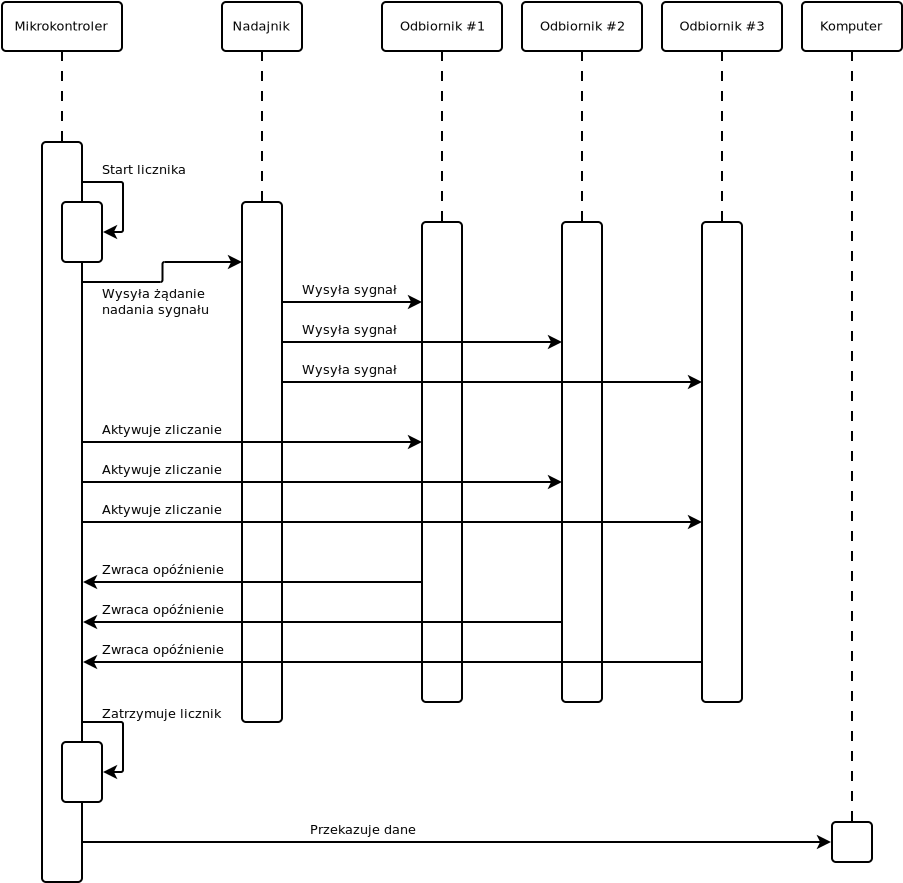
\includegraphics[width=45em]{gfx/diagramy/diagram_sekwencji_sprzetu}
 \caption{Diagram sekwencji oprogramowania mikrokontrolera}
 \label{fig:firmware_sequence_diagram}
\end{figure}

\section{Oprogramowanie dla komputera}
\subsection{Trilaterator}
Pierwsza ze stworzonych aplikacji przeznaczona jest do przeprowadzania trilateracji, o której mowa w sekcji \ref{par:trilateration}. Wykonuje ona automatycznie obliczenia dane wzorami \ref{eq:trilateration_final_x}, \ref{eq:trilateration_final_y} i \ref{eq:trilateration_final_z}. Interfejs aplikacji umożliwia wprowadzanie wszelkich danych dotyczących rozmieszczenia odbiorników jak i markera.

Aplikację prezentuje rysunek \ref{fig:trilaterator}.

\begin{figure}
 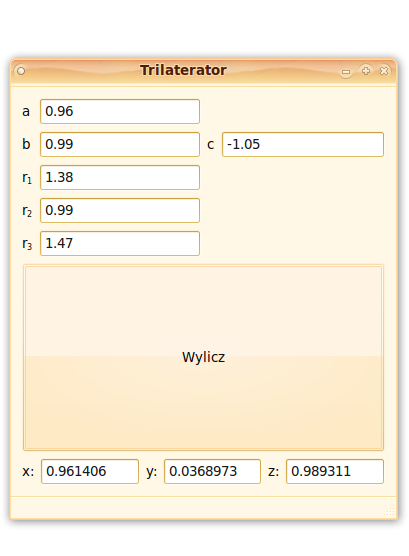
\includegraphics[width=\textwidth]{gfx/trilaterator}
 \caption{Trilaterator. Aplikacja dokonująca trilateracji}
 \label{fig:trilaterator}
\end{figure}

\subsection{Charter}
Kolejna aplikacja prezentująca możliwości systemu służy do rysowania wykresów w czasie rzeczywistym na podstawie danych pobranych z mikrokontrolera. Dla porównania dostępne są dwa rodzaje wykresów jednocześnie:
\begin{itemize}
 \item odległość od odbiornika \ppauza pokazuje odległość wybranego markera od każdego z odbiorników,
 \item położenie \ppauza dokonuje w locie trilateracji dla bieżącej próbki i rysuje wykres położenia wybranego markera w trzech wymiarach.
\end{itemize}

Odległość od odbiorników podawana jest jako wartość licznika odczytana z mikrokontrolera. Aby dokonać konwersji na centymetry, należy (w oparciu o równanie \ref{eq:microcontroller_limit}) przeliczyć:
\begin{equation}
 d = \frac{x * 0.34\textrm{mm}}{10}
\end{equation}
gdzie:
\begin{description}
 \item[$d$] \ppauza~wyznaczona odległość w centymetrach,
 \item[$x$] \ppauza~odległość odczytana z wykresu.
\end{description}

Program dokonuje transformacji układu współrzędnych, aby w efekcie uzyskać układ pokazany na rysunku \ref{fig:coordinate_system}.

Jest to taki sam układ, jak wykorzystywany w bibliotece \textsc{OpenGL}, co znacząco ułatwia pracę, ponieważ nie jest wymagana żadna dodatkowa konwersja układu współrzędnych aby narysować pozycję markera.

\begin{figure}
 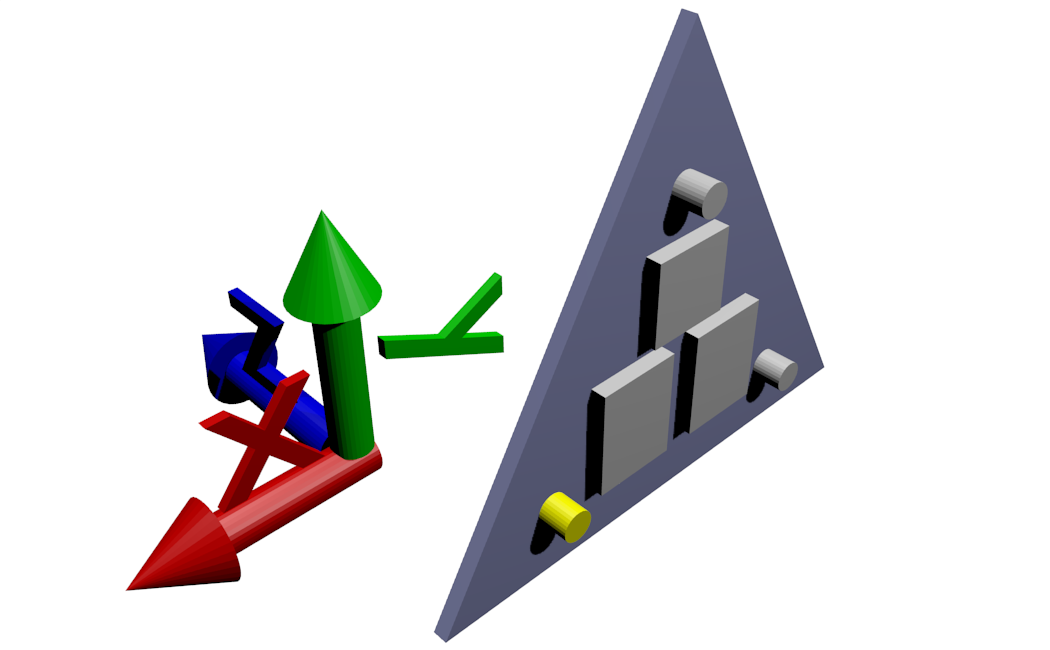
\includegraphics[width=\textwidth]{gfx/uklad_render.png}
 \caption[Model systemu i przyjęty układ współrzędnych]{Model systemu wraz z przyjętym układem współrzędnych. Układ ma swój początek w odbiorniku oznaczonym kolorem żółtym}
 \label{fig:coordinate_system}
\end{figure}

\section{Protokół}
Mikrokontroler komunikuje się z komputerem za pomocą standardu \textsmaller{RS232}, do obsługi którego wykorzystuje moduł \textsmaller{USART}\graffito{do indeksu i jeszcze raz wystepuje}. Aby uzgodnić dane pomiędzy komputerem a mikrokontrolerem, zaprojektowałem protokół, zgodnie z którym następuje przekazanie danych.

Protokół taki powinien zawierać możliwie mało nadmiarowych danych, umożliwiać synchronizację bez względu na moment włączenia nadajnika (mikrokontrolera) względem odbiornika (komputera) oraz zawierać wszystkie potrzebne informacje do odtworzenia położenia wszystkich obsługiwanych markerów.

Ramkę zaprojektowanego protokołu prezentuje rysunek \ref{fig:protocol}.

\begin{figure}
 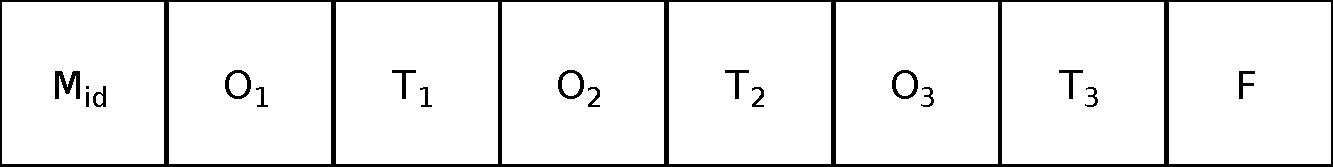
\includegraphics[width=\textwidth]{gfx/diagramy/protokol}
 \caption{Protokół komunikacji mikrokontrolera z komputerem}
 \label{fig:protocol}
\end{figure}

Każda ramka składa się z ośmiu bajtów, do których należą:
\begin{itemize}
 \item \texttt{M$_\textrm{\texttt{id}}$} \ppauza $id$ markera,
 \item \texttt{O$_n$} \ppauza wartość zmiennej \texttt{ovfCounter} w chwili wygaszenia pinu odbiornika $n$,
 \item \texttt{T$_n$} \ppauza wartość rejestru \texttt{TCNT0} w chwili wygaszenia pinu odbiornika $n$,
 \item \texttt{F} \ppauza zawsze \texttt{0xFF}.
\end{itemize}

Pole \texttt{F} wraz z polem \texttt{M$_\textrm{\texttt{id}}$} służy do synchronizacji danych odbieranych przez komputer. Metodę synchronizacji prezentuje algorytm \ref{alg:sync}.

\begin{algorithm}
\caption{Metoda synchronizacji danych}
\label{alg:sync}
\begin{algorithmic}[1]
  \REQUIRE $n \geq 0 \vee x \neq 0$
  \WHILE{\texttt{dane.count() $\geq$ 8}}
    \WHILE{\texttt{dane.count() $\geq$ 8 \&\& (dane[0] != M$_\textrm{\texttt{id}}$ \textbar{}\textbar{} dane[7] != 0x77})}
      \STATE usuń(\texttt{dane[0]})
    \ENDWHILE
  \ENDWHILE
\end{algorithmic}
\end{algorithm}